
\section{Einführung}

Die Vorliegende Dokumentation enthält die verschiedenen \LaTeX -Elemente für das Benutzerhandbuch von CUBE ProjectAssistant.
Die Befehle basieren auf den eingebundenen Paketen in der Hauptdatei (CUBEPA\_Handbuch.tex). Nachfolgend gesamter Header der Datei mit den Einstellungen:


\begin{scriptsize}
\begin{verbatim}
\documentclass[12pt]{article} % Default font size is 12pt, it can be changed here

\renewcommand{\familydefault}{\sfdefault} % Standardfont ändern auf Sans Se rif (bny)

\usepackage[left=3cm,right=2.5cm,top=2.5cm,bottom=3cm]{geometry} % Required to change the page size to A4
% manuelle Seitenränder eingesetzt durch bny einfach alles inkl. [] wieder löschen, 09.04.2016
\geometry{a4paper} % Set the page size to be A4 as opposed to the default US Letter

\usepackage[utf8x]{inputenc}
\usepackage[german]{babel} % Sprache umschalten /hat funktioniert bis auf Authors, bny 13.04.2016
\usepackage{graphicx} % Required for including pictures
\usepackage{graphics} % Möglichkeit Bilder im Textfluss einzubinden - bny / 09.04.2016
\usepackage{float} % Allows putting an [H] in \begin{figure} to specify the exact location of the figure
\usepackage{wrapfig} % Allows in-line images such as the example fish picture
\usepackage[dvipsnames]{xcolor} % von bny hinzugefügt
\usepackage{paralist} % Aufzählung mit weniger Abstand - bny
\usepackage[bookmarksopen=true,colorlinks,linkcolor = black]{hyperref} % Hinzugefügt am 21.04.2016 - bny
\usepackage{adjustbox} % Bild/Text ausrichten; hinzugefügt am 21.04.2016, bny
\usepackage{eurosym}
\usepackage{xcolor} % für Textbox mit Farbhintergrund, bny 09.11.2018
\usepackage{mdframed} % für Textbox mit Farbhintergrund, bny 09.11.2018

\linespread{1.2} % Line spacing
%\setlength\parindent{0pt} % Uncomment to remove all indentation from paragraphs
\graphicspath{{Pictures/}} % Specifies the directory where pictures are stored
\setlength{\parindent}{0pt} % Neue Absätze nicht einrücken - bny 09.04.2016

\newcommand{\HRule}{\rule{\linewidth}{0.5mm}} % Defines a new command for the horizontal lines, change thickness here
\newcommand{\col}[1]{\textbf{\textcolor[rgb]{0.4392157,0.1882353,0.627451}{#1}}}

\end{verbatim}
\end{scriptsize}

% +++++++++++++++++++++++++++++++++++++++++++++++++++++++++++++++++++++++++++++

\pagebreak
\section{Dokumentation}

% +++++++++++++++++++++++++++++++++++++++++++++++++++++++++++++++++++++++++++++

\subsection{Grundeinstellungen}

\textbf{Grafik-Pfad:}
\begin{verbatim}
\graphicspath{{Pictures/}}
\end{verbatim}


% +++++++++++++++++++++++++++++++++++++++++++++++++++++++++++++++++++++++++++++

\subsection{Text Format}

\textbf{Text in Fett:}\\ Beispiel: \textbf{Dieser Satz ist fett.}\\ Code: \verb+\textbf{Dieser Satz ist fett.}+

\vspace{\baselineskip}

\textbf{Text in Kursiv:}\\ Beispiel: \textit{Dieser Satz ist kursiv.}\\ Code: \verb+\textit{Dieser Satz ist kursiv.}+

\vspace{\baselineskip}

\textbf{Textgrössen:}
Beispiel kleiner Text:
\begin{small}
Dieser Text ist klein.
\end{small}

Code:
\begin{verbatim}
\begin{small}
Dieser Text ist klein.
\end{small}
\end{verbatim}

Alternativ kann Text direkt verkleinert werden: \small{Dieser Text ist nun klein.} \normalsize{}

\vspace{\baselineskip}

Code: \verb+\small{Dieser Text ist nun klein.}+

\vspace{\baselineskip}

Folgender Link zeigt eine Übersicht über die verschiedenen Textgrössen: \href{https://de.overleaf.com/learn/latex/Font_sizes,_families,_and_styles}{\color{blue} Schriftgrössen}  

\vspace{\baselineskip}

\textbf{Text in Anführungsstrichen:}\\
Schaltflächen, welche ohne Grafik dargestellt werden oder Menüpunkte und ähnliches werden in \textbf{' x '} dargestellt. Wichtig ist zu beachten, dass exakt diese Zeichen verwendet werden müssen. Ansonsten intepretiert \LaTeX \enspace unter Umständen andere Funktionen.

\vspace{\baselineskip}

\textbf{Farbiger Text:}

Beispiel:\\
\textcolor{NavyBlue}{Text}

Code:

\begin{verbatim}
\textcolor{NavyBlue}{Text}
\end{verbatim}

\vspace{\baselineskip}

\textbf{Farbige Textboxen (können auch Grafiken enthalten):}\\
(es wurde dazu zwei Pakete installiert)

Beispiel:
\begin{mdframed}[backgroundcolor=orange!30] 
Text (inkl. Fett, Bilder etc...)
\end{mdframed}

Code:
\begin{verbatim}
\begin{mdframed}[backgroundcolor=orange!30] 
Text (inkl. Fett, Bilder etc...)
\end{mdframed}
\end{verbatim}



% +++++++++++++++++++++++++++++++++++++++++++++++++++++++++++++++++++++++++++++

\subsection{Verweise und Links}

\textbf{Verweise innerhalb des Dokuments:}

\begin{compactitem}
	\item Zielverweise (Hierhin soll verknüpft werden - z.B. Anfangs Kapitel)- Code kommt zum Beispiel unter \verb+\section+: \verb+\label{bkm:Ref2019041801}+
	\item Befehlsverweise (Von da nach Zielverweis - meistens Ref. im Text): \verb+\ref{bkm:Ref2019041801}+
\end{compactitem}

\vspace{\baselineskip}

Nummernbildung: Grundsätzlich kann der Verweis eine beliebige Nummerierung beinhalten. Es gibt im Dokument auch verschiedene Ansätze. Jedoch wird empfohlen folgende Logik zu verwenden: -Jahr-Monat-Tag-Laufnummer, bestehend aus 2 oder 3 Ziffern. So sollte sichergestellt werden, dass keine falschen Bezüge im Dokument hinterlegt werden. Beispiel siehe oben.

\vspace{\baselineskip}

\textbf{Farbige Links:}\\
Beispiel: {\color{red} https://cube.emchberger.ch/wb/pa}
\begin{verbatim}
Code: {\color{red} https://cube.emchberger.ch/wb/pa}
\end{verbatim}
Die Farbpalette ist unter {\color{blue} https://www.namsu.de/Extra/pakete/Xcolor.html} zu finden.

\vspace{\baselineskip}

\textbf{Links:}

Beispiel: \href{www}{\color{blue} Linkname}

\begin{verbatim}
Code: \href{www}{\color{blue} Linkname}
\end{verbatim}

\verb+\color{blue}+ kann auch gelöscht werden.




% +++++++++++++++++++++++++++++++++++++++++++++++++++++++++++++++++++++++++++++
\pagebreak
\subsection{Grafiken}

\textbf{Icons / Grafiken im Text platzieren:}\\

Beispiel:
Dieses Icon 
\includegraphics[height=12pt]{/Icons/Gruppe.jpg} ist im Text eingebunden.

\vspace{\baselineskip}

Code: \verb+\includegraphics[height=12pt]{/Icons/menu.jpg}+

\begin{compactitem}
	\item Icons erhalten die Schriftgrösse 12.
	\item Buttons wie 'Erstellen', 'Übernehmen' etc werden mit Schriftgrösse 14 dargestellt.
\end{compactitem}

\vspace{\baselineskip}

\textbf{Bilder in halber Breite:}

Beispiel:

\begin{figure}[H]
\center{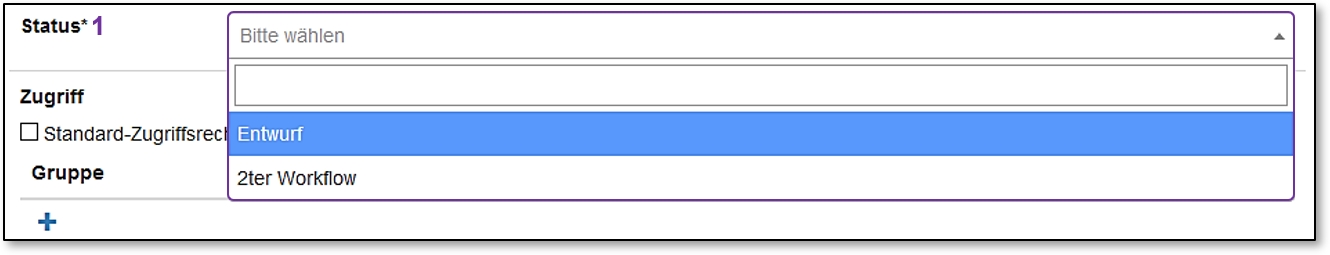
\includegraphics[width=0.5\linewidth]{../pictures/Printscreen.jpg}}
\caption{Printscreen in halber Breite}
% \label{fig:speciation}
\end{figure}

Code:

\begin{verbatim}
\begin{figure}[H]
\center{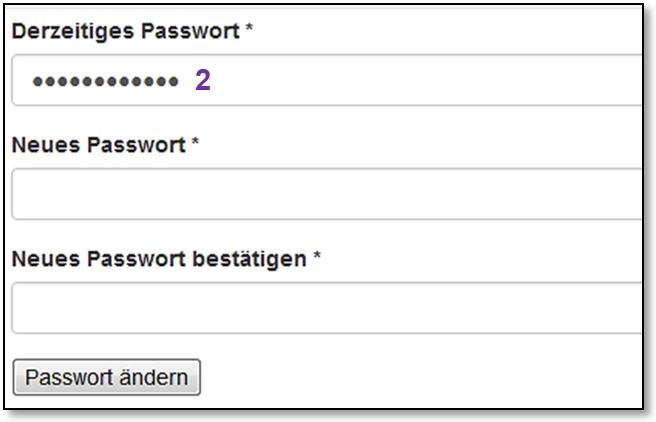
\includegraphics[width=0.5\linewidth]{../pictures/24_PWFelderausf.jpg}}
\caption{Das Menü in CUBE PA}
% \label{fig:speciation}
\end{figure}
\end{verbatim}

\textbf{Bilder in ganzer Breite:}

Beispiel:

\begin{figure}[H]
\center{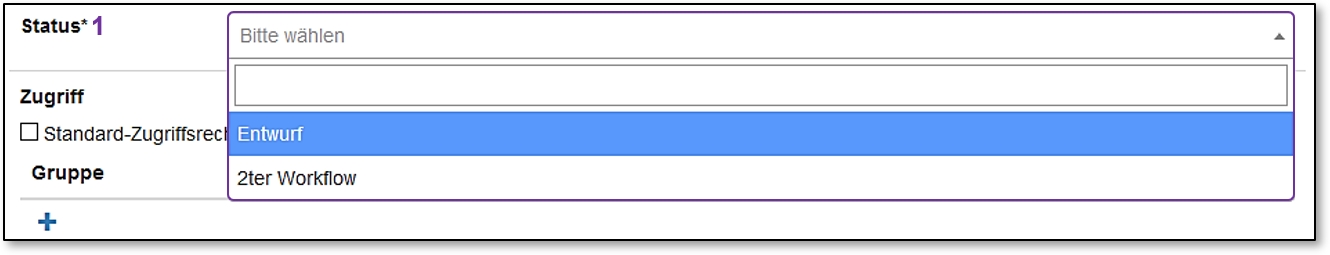
\includegraphics[width=1\linewidth]{../pictures/Printscreen.jpg}}
\caption{Printscreen in ganzer Breite}
% \label{fig:speciation}
\end{figure}

Code:

\begin{verbatim}
\begin{figure}[H]
\center{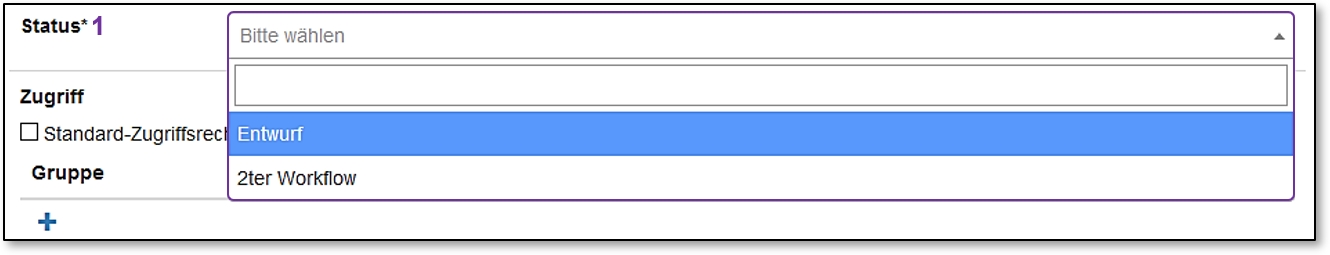
\includegraphics[width=1\linewidth]{../pictures/Printscreen.jpg}}
\caption{Passwort vergessen}
% \label{fig:speciation}
\end{figure}
\end{verbatim}

\textbf{Text und Bild nebeneinander:}

Beispiel:

\begin{wrapfigure}[7]{r}{8cm}   % [x] Wie manche Zeile soll sich um die Grafik "brechen"
  \vspace{-50pt}      % Grundwert war 20; mit 30 schön oben beim Text ausgerichtet
  \begin{center}
    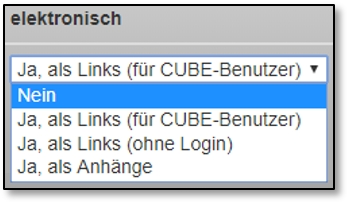
\includegraphics[height=40mm]{../pictures/Text-Bild.jpg}
  \end{center}
  \vspace{-20pt}
  \caption{Die Adressliste im Menü aufrufen}
  \vspace{-10pt}
\end{wrapfigure}

Das Bild wird rechts ausgerichtet. Mit der Option \verb+{r}+ kann definiert werden, ob das Bild rechts oder links positioniert werden soll. Zudem wird der Bildplatz angegeben \verb+{6cm}+. Wie unten erläutert, kann das Bild je nach Bedarf mit \verb+\vspace{-30pt}+ nach oben oder unten geschoben werden.

\vspace{.5cm}

Code:

\begin{verbatim}
\begin{wrapfigure}[7]{r}{6cm}   % [x] Wie manche Zeile soll sich um die Grafik "brechen"
  \vspace{-30pt}      % Grundwert war 20; mit 30 schön oben beim Text ausgerichtet
  \begin{center}
    \includegraphics[height=50mm]{../chapters/xy.jpg}
  \end{center}
  \vspace{-20pt}
  \caption{Die Adressliste im Menü aufrufen}
  \vspace{-10pt}
\end{wrapfigure}
\end{verbatim}

Im Anschluss an obigen Code erfolgt der Text.

\vspace{\baselineskip}

\textbf{Erklärungen zur Bildkonfiguration:}

\begin{compactitem}
	\item Bild in halber und ganzer Breite: bei \verb+[width=]+ wird die Grösse angegeben. 1 entspricht ganzer Breite, .5 der halben. \textbf{Beispiel:} \verb+[width=1\linewidth]+\\
	Die Massangaben können auch in mm oder cm erfolgen: \textbf{Beispiel:} \verb+[height=50mm]+
	\item Bei 'Text und Bild' nebeneinander werden in den \verb+[]+ Klammern die Anzahl Textzeilen angegeben, welche um das Bild umgebrochen werden sollen. Dies ist oft nach einfügen eines Bildes anzupassen. mit \verb+\vspace{-30pt}+ kann das Bild nach oben oder unten gerückt und so an den Text oder das Seitenlayout angepasst werden.
	\item Weitere Informationen im Internet nachschauen.
\end{compactitem}

\vspace{\baselineskip}

\textbf{Kurze Variante von 'wrap':}

\begin{verbatim}
\begin{wrapfigure}[6]{r}{6cm}
\vspace{-5pt}
\includegraphics[width=1\linewidth]{../chapters/xy.jpg}
\caption{Beschriftung}
\end{wrapfigure}
\end{verbatim}

\pagebreak
\textbf{Text - Bild - Text (nach einem langen Bild):}

Beispiel:\\
Hier steht ein Beispieltext. Hier steht ein Beispieltext. Hier steht ein Beispieltext.

\begin{center}
\hspace{-15pt}   
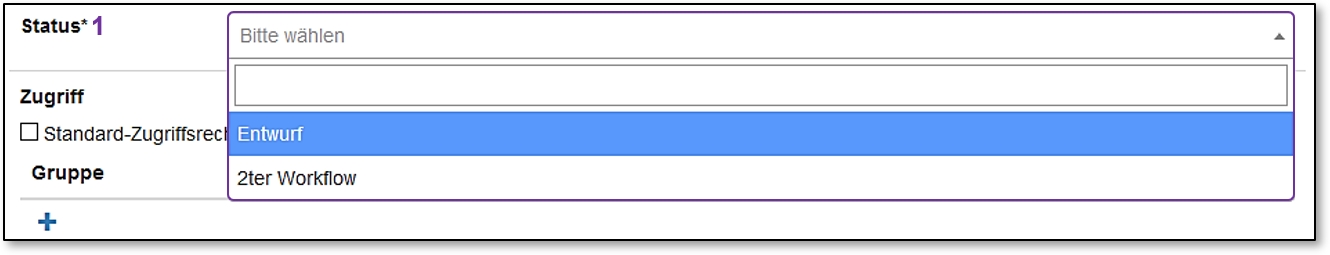
\includegraphics[width=.4\linewidth]{../pictures/Printscreen.jpg}
\end{center}

Hier steht ein Beispieltext. Hier steht ein Beispieltext. Hier steht ein Beispieltext.

\vspace{\baselineskip}

Code:

\begin{verbatim}
\begin{center}
\hspace{-15pt}   
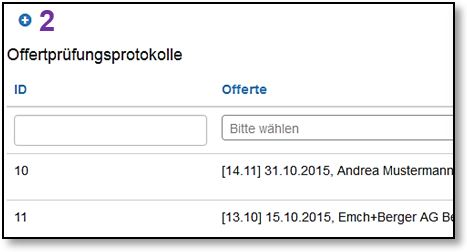
\includegraphics[width=.4\linewidth]{716_OffertpruefungsprotokollUebersicht.jpg}
\end{center}
\end{verbatim}

\textbf{Text und Bild nebeneinander (Fluss):}

Beispiel:

\begin{wrapfigure}[2]{r}{8cm}
\vspace{-45pt}
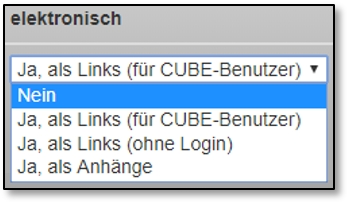
\includegraphics[height=40mm]{../pictures/Text-Bild.jpg}
% \caption{Status ändern}
\end{wrapfigure}

Hier steht ein Beispieltext. Hier steht ein Beispieltext. Hier steht ein Beispieltext. Hier steht ein Beispieltext.

\vspace{.5cm}

Code:

\begin{verbatim}
\begin{wrapfigure}[2]{r}{6cm}
\vspace{-15pt}
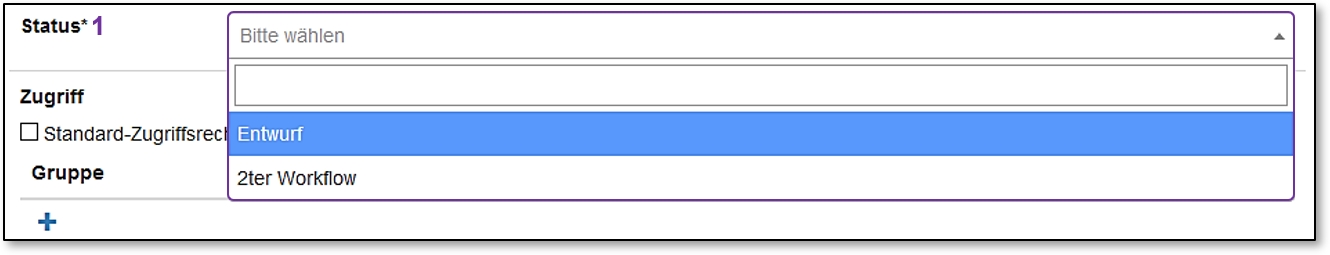
\includegraphics[height=50mm]{../pictures/Printscreen.jpg}
% \caption{Status ändern}
\end{wrapfigure}
\end{verbatim}

Mit \verb+\vspace{-15pt}+ wird das Bild gegen oben oder unten geschoben. (Beschriftung wurde deaktiviert).

\vspace{\baselineskip}

\textbf{Grafik einbinden und horizontal einschieben:}\\

Beispiel:

\hspace{15mm} 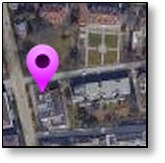
\includegraphics[height=20mm]{../pictures/kleinesBild.jpg}

Code:

\begin{verbatim}
\hspace{15mm} 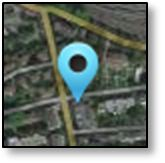
\includegraphics[height=20mm]{1123_GoogleMapNadel.jpg}
\end{verbatim}



% +++++++++++++++++++++++++++++++++++++++++++++++++++++++++++++++++++++++++++++

\subsection{Abstände und Absätze}

\textbf{Neue Seite:}
\verb+\pagebreak+ oder \verb+\clearpage+

\vspace{\baselineskip}

\textbf{Ausrichtung:}

\begin{verbatim}
\raggedright{}
\raggedleft{}
\centering{}
\end{verbatim}

Alternativ kann auch \verb+\begin+ und \verb+\end+ verwendet werden:\\
\verb+\begin{raggedleft}+ und am Ende \verb+\end{raggedleft}+.

\vspace{\baselineskip}

\textbf{Forcierter Zeilenumbruch:} \verb+\\+\\
Optional: \verb+\\[1cm]+ mit zusätzlichem Abstand

\vspace{\baselineskip}

\textbf{Text nicht umbrechen:}
\verb+\mbox{Hier steht der Text, welcher nicht umgebrochen werden soll...}+

\vspace{\baselineskip}

\textbf{Text mit weniger Umbruch:}

Der Text innerhalb dieser Funktion wendet eine grosszügigere Formatierung an. Es gibt weniger Worttrennungen am Zeilenende, die Wortabstände können grösser sein.

Code:

\begin{verbatim}
\begin{sloppypar} ... \end{sloppypar}
\end{verbatim}

\vspace{\baselineskip}

\textbf{Abstand zwischen Textblöcken und anderen Elementen:}\\
\verb+\vspace{\baselineskip}+

\vspace{\baselineskip}

\textbf{Grösserer / benutzerdefinierter Abstand:} \verb+\vspace{15cm}+ | Optional: * nach vspace*\\

Abstand 3cm:
\vspace{3cm}


\textbf{Horizontaler Abstand:} \verb+\quad+

Beispiel: \quad Abstand \quad Abstand




% +++++++++++++++++++++++++++++++++++++++++++++++++++++++++++++++++++++++++++++

\pagebreak
\subsection{Tabellen}

\textbf{Tabellen mit Icons:}
Links sind die Icons, rechts der Text mit Umbruch. Breite 14cm.\\

Beispiel:\\

\begin{tabular}{c | p{14cm} l} %{cl}

\includegraphics[height=12pt]{pictures/icons/Gruppe.jpg} & Verbindung ist unterbrochen. \\

\includegraphics[height=12pt]{pictures/icons/Gruppe.jpg} & Sie haben eine Verbindung. \\

\includegraphics[height=12pt]{pictures/icons/Gruppe.jpg} & Sie sind nicht angemeldet. \\
\end{tabular}

\vspace{\baselineskip}

Code:

\begin{verbatim}
\begin{tabular}{c | p{14cm} l} %{cl}

\includegraphics[height=12pt]{/icons/Gruppe.jpg} & Verbindung ist unterbrochen. \\

\includegraphics[height=12pt]{/icons/Gruppe.jpg} & Sie haben eine Verbindung. \\

\includegraphics[height=12pt]{/icons/Gruppe.jpg} & Sie sind nicht angemeldet. \\
\end{tabular}
\end{verbatim}

\vspace{\baselineskip}

\textbf{Rahmen und Ränder bei Tabellen werden wie folgt gemacht:}

\begin{compactitem}
	\item Mit dem Zeichen \verb+|+ (Alt Gr + 7)
	\item Mit \verb+\hline+
\end{compactitem}

\vspace{\baselineskip}

Beispiel:\\
\begin{tabular}{|c | p{10cm}|l} %{cl}
\hline
Text A & Text B \\
\hline
Text C & Test D \\
\hline
\end{tabular}

\vspace{\baselineskip}

Code:
\begin{verbatim}
\begin{tabular}{|c | p{10cm}|l} %{cl}
\hline
Text A & Text B \\
\hline
Text C & Test D \\
\hline
\end{tabular}
\end{verbatim}

\vspace{\baselineskip}


% bishierher

\textbf{Grafik in Tabellen (zentrieren - horizontal):}\\
Achtung: Klammern sind wichtig!

Beispiel:

\begin{tabular}{|c | p{10cm}|l} %{cl}
\hline
Text A & Text B \\
\hline
Text C & \raisebox{-1\totalheight}{
\includegraphics[height=20pt]{pictures/icons/Gruppe.jpg}} \\
\hline
\end{tabular}

\pagebreak
Code:

\verb+\raisebox{-1\totalheight}{
\includegraphics[height=20pt]{/Icons/B_Erstellen.jpg}}+

Achtung: allenfalls ergibt \verb+\raisebox+ (wie im Dokument angewendet) ein Error!

\vspace{\baselineskip}

$\Rightarrow$ Manueller Zeilenumbruch innerhalb von Tabellen (Spalten): \verb+\newline+\\



% +++++++++++++++++++++++++++++++++++++++++++++++++++++++++++++++++++++++++++++

\subsection{Aufzählungen und weitere Elemente}

\textbf{Normale Aufzählung - 1 Ebene:}\\

Beispiel (Mit Fett-Text):
\begin{itemize}
\item
\textbf{Übersicht}: zeigt die für Sie relevanten Sitzungen.
\item
\textbf{Adressliste:} Anzeige der erfassten Adressen.
\end{itemize}

\vspace{\baselineskip}

Code:
\begin{verbatim}
\begin{itemize}
\item
\textbf{Übersicht}: zeigt die für Sie relevanten Sitzungen.
\item
\textbf{Adressliste:} Anzeige der erfassten Adressen.
\end{itemize}
\end{verbatim}

\textbf{Aufzählungen mit 2 Ebenen:}

Beispiel:
\begin{itemize}
\item Erste Ebene
	\begin{itemize}
		\item Zweite Ebene, Punkt 1
		\item Zweite Ebene, Punkt 2
	\end{itemize}
\end{itemize}

Code:

\begin{verbatim}
\begin{itemize}
\item Erste Ebene
	\begin{itemize}
		\item Zweite Ebene, Punkt 1
		\item Zweite Ebene, Punkt 2
	\end{itemize}
\end{itemize}
\end{verbatim}

\textbf{Kompakte Aufzählung:}

Beispiel:\\
\begin{compactitem}
	\item Erster Punkt
	\item Zweiter Punkt
	\item Dritter Punkt
\end{compactitem}

\vspace{\baselineskip}

Code:

\begin{verbatim}
\begin{compactitem}
	\item Erster Punkt
	\item Zweiter Punkt
	\item Dritter Punkt
\end{compactitem}
\end{verbatim}

\vspace{\baselineskip}

\textbf{Nummerierungen:}\\
Auf den Grafiken werden immer wieder violette Nummerierungen verwendet. Um diese im Text darzustellen und aufzugreifen, wurde ein neuer Befehl kreiert:

\begin{verbatim}
\newcommand{\col}[1]{\textbf{\textcolor[rgb]{0.4392157,0.1882353,0.627451}{#1}}}
\end{verbatim}

Im Text selbst wird dieser mittels \verb+\col{(1)}+ erstellt: \col{(1)}

\vspace{\baselineskip}

\textbf{'Grösser als' / 'Kleiner als' darstellen:}

Beispiel:\\
\textgreater \quad \textless

Code: \verb+\textgreater+ \quad \verb+\textless+

\vspace{\baselineskip}

\textbf{Pfeile:}

Pfeile in \verb+$$+ darstellen.\\

Beispiel: $\Rightarrow$ Text 

Code: \verb+$\Rightarrow$+ Text

\vspace{\baselineskip}

Mehr zu Pfeilen siehe: http://www.latex-pfeile.de





% +++++++++++++++++++++++++++++++++++++++++++++++++++++++++++++++++++++++++++++

\pagebreak
\section{Hinweise} 

\begin{compactitem}
	\item Werden kundenspezifische Grafiken verwendet ist das mit der Kommentarfunktion \% zu dokumentieren.
	\item Nach einem Schriftgrössen-Wechsel kann es vorkommen, dass dann die kleinere oder grössere Schrift bleibt. In diesem Fall ist manuell wieder auf die gewünschte Schrift zurückzustellen, z.B. mit \verb+\normalsize{}+
	\item nach einem verwendeten \LaTeX \enspace bleibt ein Space aus, dieses kann mittels \verb+\enspace+ eingefügt werden.

\end{compactitem}

\vspace{\baselineskip}
\vspace{\baselineskip}

% +++++++++++++++++++++++++++++++++++++++++++++++++++++++++++++++++++++++++++++


\section{Übersicht über vorhandene Handbücher, Dokumentationen und Informationen}


\begin{itemize}
	\item \textbf{\LaTeX-Handbuch:} in Deutsch, Französisch* und Englisch*
	\item \textbf{Quick-Ref:} Kurzanleitungen von verschiedenen Modulen oder Funktionen.
	\item \textbf{Upgrade-Info:} Es sind Upgrade-Informationen von Version 2.7 zu 2.11 und von Version 2.11 zu 2.12 vorhanden. Diese Informationen wurden generisch und teils kundenspezifisch erstellt.
\end{itemize}

\vspace{\baselineskip}

* Das französische und englische Handbuch ist nicht mehr auf dem aktuellen Stand

\vspace{\baselineskip}

\textbf{Hinweis:} Beim \LaTeX-Handbuch werden in allen Sprachen die deutschen Printscreens verwendet.


